\hypertarget{procesoCompra}{}
\section{Proceso 1: Comprar}

\subsection{Resumen del proceso}
	El proceso de comprar define la serie de acitividades que son necesesarias para que un cliente pueda comprar uno o m\'as articulos dentro de SpaceShop. \\
	
\subsection{Actores que participan en el proceso}
	\hyperlink{Cliente}{Cliente} \\
	
\subsection{Diagrama de proceso}
	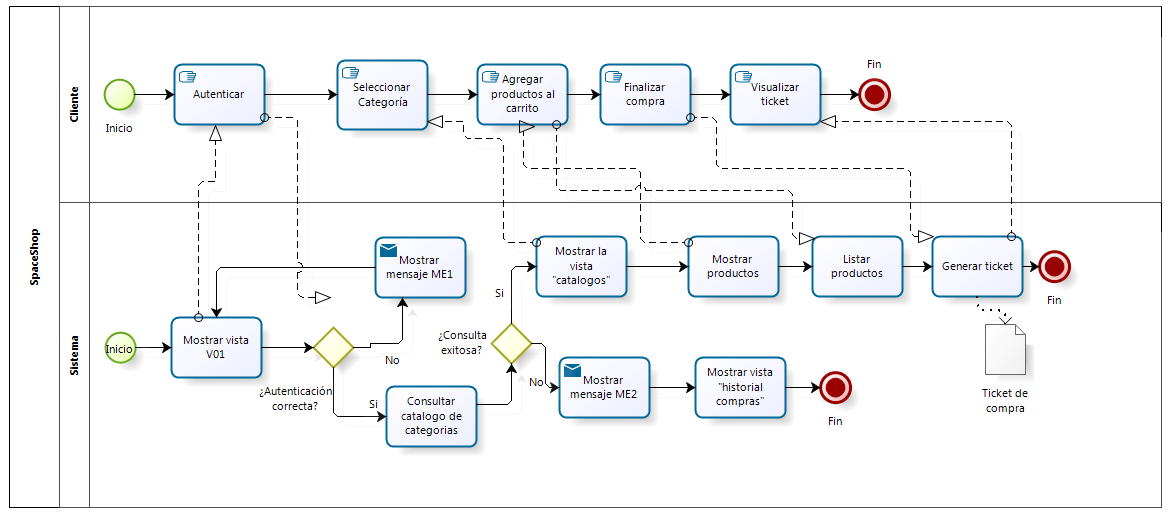
\includegraphics[scale=0.60]{images/procesos/ProcesoComprar.png}
	\\ \\
\subsection{Objetivo General}
	Realizar una compra dentro de SpaceShop. 
	
\subsubsection{Objetivos Particulares}
	\begin{enumerate}
		\item Consultar y visualizar la existencia de los articulos.
		\item Mostrar las categorias registradas en el sistemas as\'i como los articulos relacionados a estas.
		\item Generar un ticket de la compra generada.
	\end{enumerate}
	
\newpage	
\subsection{Insumos de entrada}
	\begin{enumerate}
		\item Identificador del articulo seleccionado.
		\item N\'umero de articulos que se desean agragar al carrito de compras.
	\end{enumerate}
	
\subsection{Elementos de entrada}
	\begin{enumerate}
		\item Petici\'on para mostrar las categorias existentes en la tienda.
		\item Petici\'on para mostrar el catalogo de productos de la categoria seleccionada.
		\item Petici\'on para generar el ticket de compra.
	\end{enumerate}
	
	
\subsection{Salidas}
	\begin{enumerate}
		\item Registro la compra realizada.
		\item Ticket generado por la compra efectuada.
	\end{enumerate}
	
	
\subsection{Clientes o consumidores}
	\begin{enumerate}
		\item \hyperlink{Cliente}{Cliente}
	\end{enumerate}
	
	
\subsection{Mecanismos de medici\'on}
	\begin{enumerate}
		\item La comprobaci\'on del correcto funcionamiento del proceso.
	\end{enumerate}
	
	
\subsection{Recusos necesarios para el proceso}
	\begin{enumerate}
		\item Usuario tipo \hyperlink{Cliente}{Cliente} registrado y autenticado.
		\item Una computadora.
		\item Conexi\'on a internet.
		\item Explorador web
	\end{enumerate}
	
	
\subsection{Interacci\'on con otros procesos}
	\begin{itemize}
		\item No existe interacci\'on con otros procesos.
	\end{itemize}
	
	
\subsection{Tipos de solicitud que ejecuta el proceso}
	\begin{itemize}
		\item Solicitud emitida por el \hyperlink{Cliente}{Cliente}.
	\end{itemize}

\newpage	
\subsection{Descipci\'on de las actividades}
\textit{\\}
	\begin{enumerate}
		\item Autenticar: El cliente deber\'a ingresar los datos en la vista \hyperlink{V01}{V01} tal como los especifica la \hyperlink{RN001}{RN001}. \\
		
		\item Seleccionar Categoria: El usuario dara clic en la imagen de la categoria que desea comprar dentro de la vista categorias. \\
		
		\item Agregar productos al carrito: El \hyperlink{Cliente}{Cliente} seleccionar\'a los productos que desee comprar as\'i como la cantidad que desea de cada articulo.  \\
		
		\item Finalizar compra: El \hyperlink{Cliente}{Cliente} dar\'a clic en el bot\'on Terminar compra en la vista carrito para confirmar que desea finalizar su compra. \\
		
		\item Visualizar ticket: El \hyperlink{Cliente}{Cliente} dar\'a clic en el bot\'on "Visualizar ticker" en la vista \hyperlink{V02}{"V02"}. \\
		
		\item Mostrar vista V01: El sistema mostrar\'a al \hyperlink{Cliente}{Cliente} la vista de autenticaci\'on \hyperlink{V01}{"V01"}. \\
		
		\item Mostrar mensaje ME1: El sistema mostrar\'a el mensaje \hyperlink{ME1}{ME1} con la vista \hyperlink{V03}{"V03"}. \\
		
		\item Consultar catalogos de categorias: El sistema realizar\'a una consulta ha la base de datos para obtener las categor\'ias registradas. \\
		
		\item Mostrar la vista "catalogos": El sistema mostrar\'a la vista de \hyperlink{catalogos}{"catalogos"} con el resultado de la consulta realizada. \\
		
		\item Mostrar mensaje ME2: El sistema mostrar\'a el mensaje \hyperlink{ME2}{ME2} a trav\'es de la vista \hyperlink{V04}{"V04"}. \\
		
		\item Mostrar productos: La vista \hyperlink{listado}{"listado"} mostrar\'a los productos con su una imagen, precio, su nombre y un bot\'on para agregar los productos al carrito de compras. \\
		
		\item Listar productos: El sistema recibir\'a el "Id" del producto agregado al carrito y lo guardar\'a temporalmente para despu\'es almacenar la compra creada. \\
		
		\item Generar ticket de compra: Se generar\'a un archivo PDF para mostrar la descripci\'on del \hyperlink{carrito}{carrito} generado por el cliente, los datos de la compra se almacenaran en la base de datos y se mostrar\'a la vista \hyperlink{index}{index}. \\
	\end{enumerate}